\section{Case Studies}
\label{sec:casestudies}

The random generation framework presented throughout this paper allows us to
write extensible generators in a very concise way.
%
However, this expressiveness comes attached to a perceptible runtime overhead,
primarily inherited from the use of Data Types \`a la Carte---a technique which
is not often scrutinized for performance.
%
In this section, we evaluate the implicit cost of composing generators using
three real-world case studies.


As we have shown in Section \ref{sec:generators}, the random generation
process we propose in this paper can be seen as having two phases.
%
First, we generate random values from the representation types used to specify
the shape of our data; and then we use their algebras to translate them to the
corresponding values of our target data types.
%
In particular, the transformation step is expected to pattern match repeatedly
against the |InL| and |InR| constructors of the |oplus| operators when
traversing each construction injection.
%
Because of this, in general, we expect a performance impact with respect to
manually-written concrete generators.


As recently analyzed by \citeauthor{KiriyamaOptimizingDTC}, this slowdown is
expected to be linear in the depth of our representation type
\cite{KiriyamaOptimizingDTC}.
%
In this light, one can drastically reduce the runtime overhead by associating
each |oplus| operator in a balanced fashion.
%
So, for instance, instead of writing |(f oplus'' g oplus'' h oplus'' i)|, which
is implicitly parsed as |(f oplus'' (g oplus'' (h oplus'' i)))|; we can
associate constructions as |((f oplus'' g) oplus'' (h oplus'' i))|, thus
reducing the depth of our representation from four to three levels and, in
general, from a $\mathcal{O}(n)$ to a $\mathcal{O}(log(n))$ complexity in the
runtime overhead, where $n$ is the amount of constructions under consideration.


Later, we analyzed the performance of generating random values using three case
studies:
%
\begin{inparaenum}[(i)]
\item Red-Black Trees (RBT), inspired by Okasaki's formulation
  \cite{okasaki1999red},
\item Lisp S-expressions (SExp), inspired by the package
  \emph{hs-zuramaru}\footnote{\url{http://hackage.haskell.org/package/zuramaru}},
  and
\item HTML expressions (HTML), inspired by the \emph{html}
  package\footnote{\url{http://hackage.haskell.org/package/html}}, which follows
  the same structure as our motivating |Html| example.
\end{inparaenum}
%
The magnitude of each case study can be outlined as follows:

\begin{table}[H]
  \begin{tabular}{||c||c||c||c||c||}
    \hline
    Case Study & \#|Con| & \#|Fun| & \#|Pat| & Total Constructions \\ \hline
    \hline
    RBT        & 2       & 5       & 6       & 13                  \\ \hline
    SExp       & 6       & -       & 9       & 15                  \\ \hline
    HTML       & 4       & 132     & -       & 136                 \\ \hline
  \end{tabular}
\end{table}

These case studies provide a good combination of data constructors, interface
functions and patterns, and cover from smaller to larger numbers of
constructions.


Then, we benchmarked the execution time required to generate and fully evaluate
10000 random values corresponding to each case study, comparing both
manually-written concrete generators, and those obtained using our modular
approach.
%
For this purpose, we used the \emph{Criterion} \cite{criterion} benchmarking
tool for Haskell, and limited the maximum depth of the generated values to five
levels.
%
Additionally, our modular generators were tested using both linear and balanced
generation specifications.
%
Figure \ref{fig:times} illustrates the relative execution time of each case
study, normalized to their corresponding manually-written counterpart---we
encourage the reader to obtain a colored version of this work.

\begin{figure}[t]
  \centering
  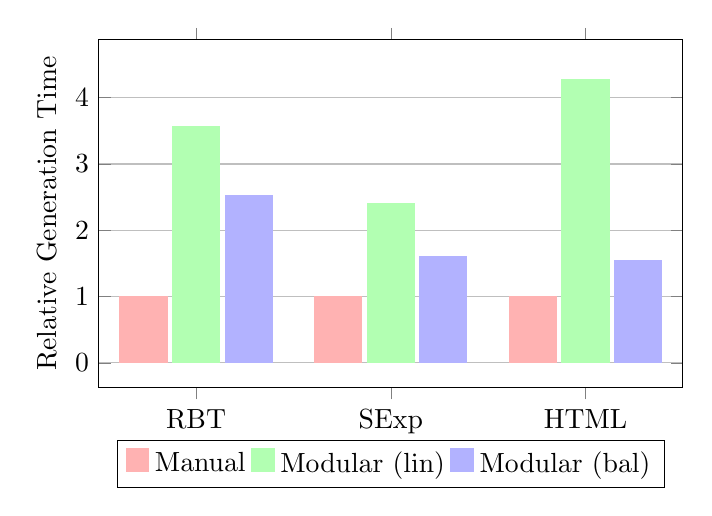
\begin{tikzpicture}
    \begin{axis}
      [ height=6cm
      , width=9cm
      , ybar
      , ymajorgrids=true
      , ytick={0,1,...,4}
      , ymax=4
      , ymin=0.5
      , enlargelimits=0.25
      , enlarge x limits=0.25
      , /pgf/bar width=17pt
      , legend style={
        at={(0.5,-0.15)},
        anchor=north,legend columns=3}
      , legend image code/.code={%
        \draw[#1, draw=none] (0cm,-0.1cm) rectangle (0.3cm,0.2cm); }
      , ylabel={Relative Generation Time}
      , symbolic x coords={RBT, SExp, HTML}
      , xtick=data
      % , nodes near coords
      , nodes near coords align={vertical}
      ]
      \addplot[fill, red!30]   coordinates {(SExp,1)    (RBT,1)    (HTML,1)};
      \addplot[fill, green!30] coordinates {(SExp,2.40) (RBT,3.57) (HTML,4.27)};
      \addplot[fill, blue!30]  coordinates {(SExp,1.60) (RBT,2.52) (HTML,1.55)};
      \legend{Manual, Modular (lin), Modular (bal)}
    \end{axis}
  \end{tikzpicture}
  \caption{Generation time comparison between concrete and modular generators.}
  \label{fig:times}
\end{figure}
%
As it can be observed, our approach suffers from a noticeable runtime overhead
when using linearly defined representations, specially when considering the HTML
case study, involving a large number of constructions in the generation process.
%
However, we found that, by balancing our representation types, the generation
performance improves dramatically.
%
At the light of these improvements, our tool includes an additional type-level
computation that automatically balances our representations in order to reduce
the generation overhead.

% and relying on more sophisticated techniques like prefix-free encodings to
% obtain optimal representations, is a undergoing path of our future work.

On the other hand, it has been argued that the generation time is often not
substantial with respect to the rest of the testing process, especially when
testing complex properties over monadic code, as well as using randomly
generated values for penetration testing
\cite{DBLP:conf/haskell/MistaRH18,grieco2017}.


All in all, we consider that these results are fairly encouraging, given that
the flexibility obtained from using our compositional approach does not produce
severe slowdowns when generating random values in practice.

% , nor explodes more than linearly as we increase the complexity of our random
% generators.
